%%%%%%%%%%%%%%%%%%%%%%%%%%%%%%%%%%%%%%%%%%%%%%%%%%%%%%%%%%%%%%%%%%%%%%%%%%%%%%%%
%2345678901234567890123456789012345678901234567890123456789012345678901234567890
%        1         2         3         4         5         6         7         8

\documentclass[letterpaper, 10 pt, conference]{ieeeconf}  % Comment this line out
                                                          % if you need a4paper
%\documentclass[a4paper, 10pt, conference]{ieeeconf}      % Use this line for a4
                                                          % paper

\IEEEoverridecommandlockouts                              % This command is only
                                                          % needed if you want to
                                                          % use the \thanks command
\overrideIEEEmargins
% See the \addtolength command later in the file to balance the column lengths
% on the last page of the document



% The following packages can be found on http:\\www.ctan.org
\usepackage{graphics} % for pdf, bitmapped graphics files
\usepackage{epsfig} % for postscript graphics files
\usepackage{mathptmx} % assumes new font selection scheme installed
\usepackage{times} % assumes new font selection scheme installed
\usepackage{amsmath} % assumes amsmath package installed
\usepackage{amssymb}  % assumes amsmath package installed

\title{\LARGE \bf
SwarmTouch
}

%\author{ \parbox{3 in}{\centering Huibert Kwakernaak*
%         \thanks{*Use the $\backslash$thanks command to put information here}\\
%         Faculty of Electrical Engineering, Mathematics and Computer Science\\
%         University of Twente\\
%         7500 AE Enschede, The Netherlands\\
%         {\tt\small h.kwakernaak@autsubmit.com}}
%         \hspace*{ 0.5 in}
%         \parbox{3 in}{ \centering Pradeep Misra**
%         \thanks{**The footnote marks may be inserted manually}\\
%        Department of Electrical Engineering \\
%         Wright State University\\
%         Dayton, OH 45435, USA\\
%         {\tt\small pmisra@cs.wright.edu}}
%}

\author{Evgeny Tsykunov$^{1}$, Roman Ibrahimov$^{2}$ and Ruslan Agishev$^{3}$% <-this % stops a space
%\thanks{*This work was not supported by any organization}% <-this % stops a space
%\thanks{$^{1}$H. Kwakernaak is with Faculty of Electrical Engineering, Mathematics and Computer Science,
%        University of Twente, 7500 AE Enschede, The Netherlands
%        {\tt\small h.kwakernaak at papercept.net}}%
%\thanks{$^{2}$P. Misra is with the Department of Electrical Engineering, Wright State University,
%        Dayton, OH 45435, USA
%        {\tt\small p.misra at ieee.org}}%
%\thanks{$^{3}$P. Misra is with the Department of Electrical Engineering, Wright State University,
%        Dayton, OH 45435, USA
%        {\tt\small p.misra at ieee.org}}%
}

\begin{document}



\maketitle
\thispagestyle{empty}
\pagestyle{empty}


%%%%%%%%%%%%%%%%%%%%%%%%%%%%%%%%%%%%%%%%%%%%%%%%%%%%%%%%%%%%%%%%%%%%%%%%%%%%%%%%
\begin{abstract}

\end{abstract}


%%%%%%%%%%%%%%%%%%%%%%%%%%%%%%%%%%%%%%%%%%%%%%%%%%%%%%%%%%%%%%%%%%%%%%%%%%%%%%%%
\section{INTRODUCTION}




\section{Drones control}

\subsection{Obstacle avoidance algorithm}

The location of drones and obstacles is given by Vicon Vantage 5 motion capture system. Every object pose is broadcasted at 60 Hz frequency and is known at each period of time. So each quadrotor is aware of the obstacles positions relative to it. Drones goal positions are commanded relatively to the human location. However if a quadrotor from the swarm is approaching the obstacle its position is corrected relatively to the obstacle pose as depicted on the fig. 1. If the drone is commanded by the human to fly inside the circular vicinity of the obstacle, the aerial vehicle will avoid the object, following the circumference, defining the obstacle boundary.
However this obstacle avoidance method requires drones to move through the arc faster in comparison with following straight line trajectory. In addition the quadrotors should perform sharp maneuvers being in points $\boldsymbol{A}$ and $\boldsymbol{B}$ of the circumference.

\begin{figure}
\centering
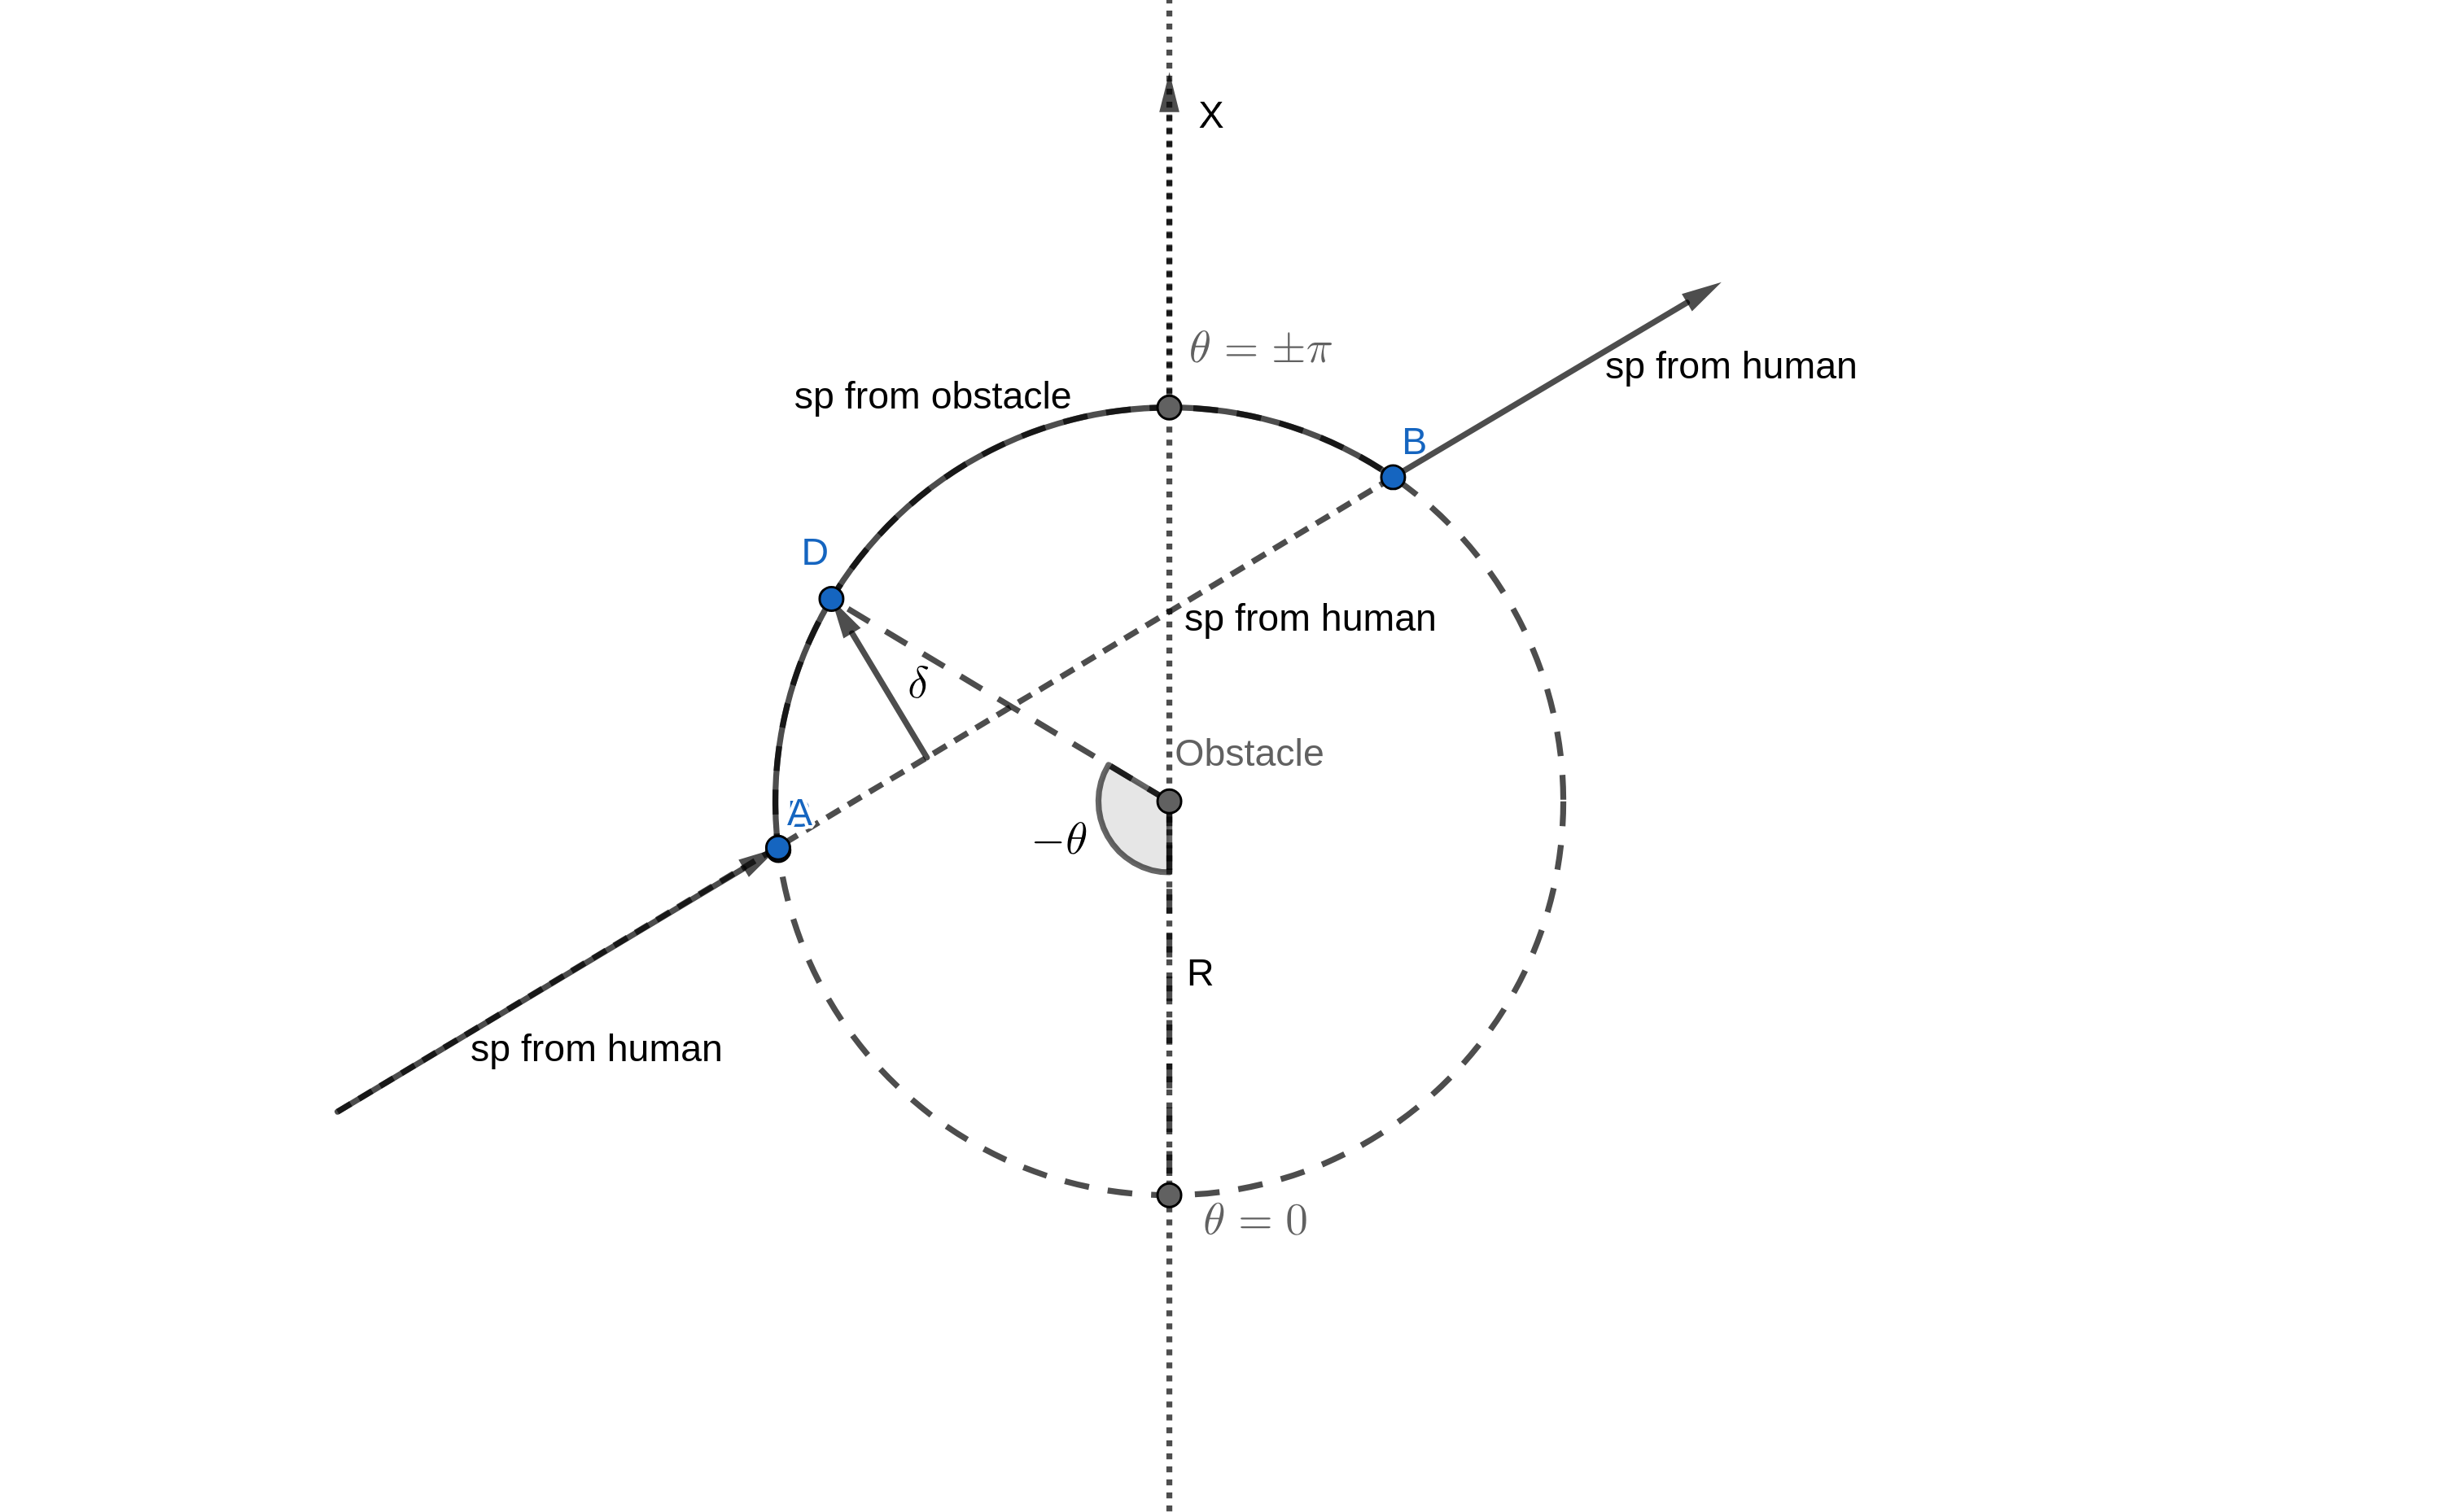
\includegraphics[width=0.5\textwidth]{figures/obstacle_avoidance.png}\label{true}
\caption{Obstacle avoidance algorithm}
\label{obstacle}
\end{figure}

\subsection{Delta-impedance control}

Impedance control is used in order to make trajectories near obstacles feasible for the drones as follows. In the circle-like obstacle vicinity the impedance correction term is added to the drone goal position, based on the distance between the set-point on the circumference and the goal position commanded by human if there were not obstacles. This distance is denoted by the letter $\delta$ on the fig. 1. In order to calculate impedance pose correction term the following equation should be solved for the drone, situated near the obstacle:
$$m\ddot{x} + b\dot{x} + k x = F_\delta (t),$$
where $F_\delta=-K\delta$, $m$ is the desired mass of virtual body, $b$ is desired damping, and $k$ is the desired stiffness. In such a way the external force $F_\delta(t)$ acting on the drone near the obstacle affects drone's desired position proportionally to $\delta$-value.
Drones trajectories in the vicinity of the obstacles become more smooth.

\subsection{Theta-impedance control}
In order to control drones angular velocities near obstacles circumferences another impedance model is implemented.
$$J\ddot{\theta} + D\dot{\theta} = M(t),$$
where $M(t) = K (\theta_{imp} - \theta_{sp})$ is a torque acting on the robot near the obstacle, $J$ is an inertia moment of the drone, and $D$ is damping coefficient. The impedance model choice is explained by damped convergence of the set-point of the drone to desired position $(R, \theta_{imp})$, expressed in polar coordinates relatively to the obstacle. 

\addtolength{\textheight}{-12cm}   % This command serves to balance the column lengths
                                  % on the last page of the document manually. It shortens
                                  % the textheight of the last page by a suitable amount.
                                  % This command does not take effect until the next page
                                  % so it should come on the page before the last. Make
                                  % sure that you do not shorten the textheight too much.

%%%%%%%%%%%%%%%%%%%%%%%%%%%%%%%%%%%%%%%%%%%%%%%%%%%%%%%%%%%%%%%%%%%%%%%%%%%%%%%%



%%%%%%%%%%%%%%%%%%%%%%%%%%%%%%%%%%%%%%%%%%%%%%%%%%%%%%%%%%%%%%%%%%%%%%%%%%%%%%%%



%%%%%%%%%%%%%%%%%%%%%%%%%%%%%%%%%%%%%%%%%%%%%%%%%%%%%%%%%%%%%%%%%%%%%%%%%%%%%%%%




%\begin{thebibliography}{99}

%\bibitem{c1} G. O. Young, ÒSynthetic structure of industrial plastics (Book style with paper title and editor),Ó 	in Plastics, 2nd ed. vol. 3, J. Peters, Ed.  New York: McGraw-Hill, 1964, pp. 15Ð64.



%\end{thebibliography}




\end{document}
